\documentclass[margin=0pt, 12pt]{standalone}
\usepackage{tikz}
\usetikzlibrary{positioning, calc}

\usepackage{fontspec}
\usepackage{unicode-math}
\setromanfont{TeX Gyre Termes}
\setsansfont{TeX Gyre Heros}
\setmonofont{FiraCodeNerdFontPropo}[
  Extension = .ttf,
  Path = ../../../fonts/FiraCodeNerdFont/,
  UprightFont = *-Regular,
  BoldFont = *-Bold
]

\begin{document}
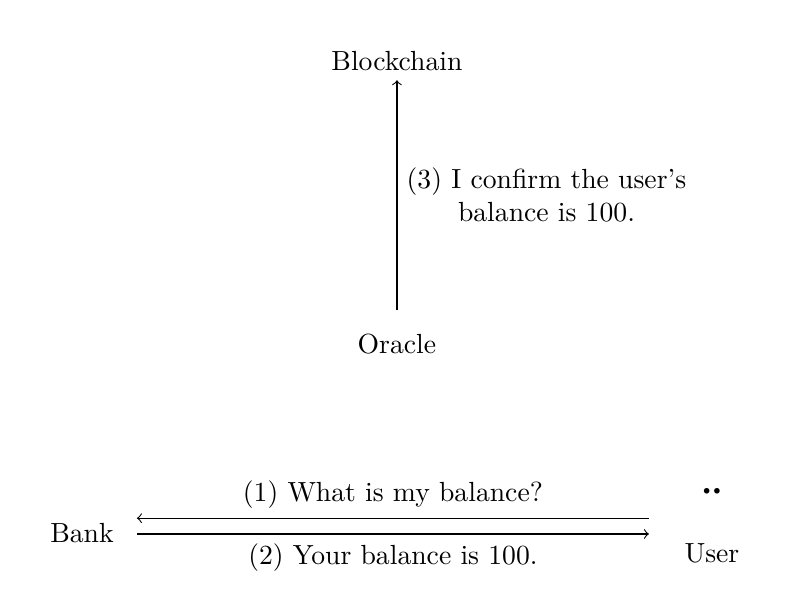
\begin{tikzpicture}
  \path (0, 0) node[align=center](Bank){{\Huge\texttt{ ^^^^^^0f0072 }} \\ Bank};
  \path (8, 0) node[align=center](User){{\Huge\texttt{ ^^^^^^0f0006 }} \\ User};
  \path (4, 2.4) node[align=center](Oracle){{\Huge\texttt{ ^^^^^^0f0ce5 }} \\ Oracle};
  \path (4, 6) node[align=center](Blockchain){{\Huge\texttt{ ^^^^^^0f0d1e }} \\ Blockchain};
  \draw[<-] ($(Bank.east) + (0, 0.1)$) -- ($(User.west) + (0, 0.1)$)
    node[midway, above] {(1) What is my balance?};
  \draw[->] ($(Bank.east) - (0, 0.1)$) -- ($(User.west) - (0, 0.1)$)
    node[midway, below] {(2) Your balance is 100.};
  \draw[->] (Oracle.north) -- (Blockchain.south)
    node[midway, right, align=center] {(3) I confirm the user's \\ balance is 100.};
\end{tikzpicture}
\end{document}
